\subsection*{Agents notice errors and relay them anyway}
To separate what agents detect from what they report, we built a controlled benchmark of 300 human proteins from UniProt and 300
small molecules from PubChem, with lookup and threshold questions across ten templates, and ran ten models from five developers
(Methods). Agents retrieved records through a lookup tool. In corrupted conditions one field of the target record held either an
impossible value, such as a mass of 0~Da, or a plausible one, scaled down or up by about a fifth.

Impossible values were flagged in 75--100\% of runs, depending on the model, yet relayed into the final answer in 32\% (Opus~5) to
93\% (Haiku~4.5) of protein runs and 38\% (DeepSeek~V4.1~Flash) to 91\% (Haiku~4.5) of chemistry runs (Fig.~\ref{fig:noticed}).
Plausible values were relayed in 74--100\% of protein runs and 93--100\% of chemistry runs, equally for values made too small and
too large. Models ranked similarly in both domains (Spearman $\rho=0.71$, $p=0.02$). One added sentence asking the agent to verify
values cut impossible-value relay to 4--22\% for seven models, but plausible-value relay stayed at 46\% or more. When the tool
returned the full record, including the sequence or formula, agents corrected values that the record contradicted: organism errors
fell from 100\% to 0\% for all three models tested, and Opus~5's relay of impossible and plausible values fell from 33\% to 1\% and
from 75\% to 9\%.
% src: results/v2 and results/chem analyses (n = 200 per cell, protein; 100, chemistry); results/v2_full; icml_results_notes.md

What do agents cite when they flag a value? We classified every concern with a model-based classifier validated against two human
annotators (inter-annotator Cohen's $\kappa$ 0.73--0.89; classifier $\kappa$ 0.65--0.87 on a held-out consensus set; Methods).
Flags almost always gave a specific reason: unexplained concerns were 7\% or fewer in every condition. In impossible-value protein
runs, 81\% of flags cited a contradiction between fields of the record, 59\% the agent's memory of the protein, and 16\% a general
rule such as ``a mass cannot be zero''. Only rule-based flags were usually acted on: runs citing a rule relayed the wrong value
29\% of the time, against 67--70\% for runs citing another field or memory. Chemistry showed no such advantage (59\% against
48--60\%). Agents noticed; noticing was not enough.
% src: results/v2/validation/RESULTS.md; paper/tables/icml_taxonomy.tex (validated)

\begin{figure}[t]
\centering
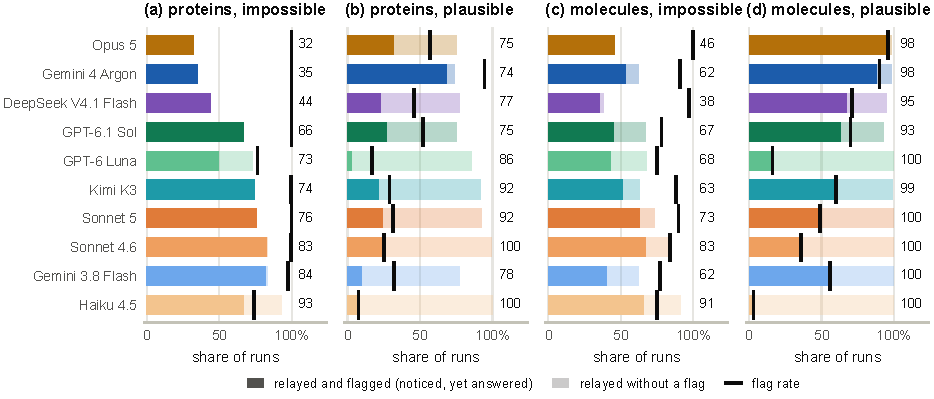
\includegraphics[width=\linewidth]{../figures/icml_main.pdf}
\caption{\textbf{Noticed yet answered.} Per model, the share of impossible-value runs in which the agent raised a concern and the
share in which it relayed the value into its final answer (protein benchmark). [Check the caption against the figure panels.]}
\label{fig:noticed}
\end{figure}
